\documentclass{article} % For LaTeX2e
\usepackage{neurips,times}
\usepackage{hyperref}
\usepackage{url}
\usepackage{booktabs}       % professional-quality tables
\usepackage{graphicx}
\usepackage{lipsum}
\usepackage{hyperref}
\usepackage{amsmath}
\usepackage{sidecap}
\usepackage{multirow}
\usepackage{siunitx}
\usepackage{pgfplots}
\pgfplotsset{compat=newest}

\usepackage[utf8]{inputenc} % allow utf-8 input
\usepackage[T1]{fontenc}    % use 8-bit T1 fonts
\usepackage{hyperref}       % hyperlinks
\usepackage{url}            % simple URL typesetting
\usepackage{booktabs}       % professional-quality tables
\usepackage{amsfonts}       % blackboard math symbols
\usepackage{nicefrac}       % compact symbols for 1/2, etc.
\usepackage{microtype}      % microtypography
\usepackage{amssymb,amsmath,bm}
\usepackage{color,soul}
\usepackage{multirow}
\usepackage{mathtools}

\newcommand{\figref}[1]{\figurename~\ref{#1}}
\usepgfplotslibrary{groupplots}


\def\figwidth{.5\linewidth}
\def\figheight{.15\textheight}
%\newlength{\figwidth}{\mywidth}
%\newlength{\figheight}{.2\textheight}


\usepackage[numbers]{natbib}
\setlength{\bibsep}{0.0pt}

\title{Predicting the Solar Potential of Rooftops using
	Image Segmentation and Structured Data\\ \vspace{0.5cm}\large{Report}}
\author{Stefan Wezel \\ stefan.wezel@student.uni-tuebingen.de \\4080589  \\ ML4S}

\newcommand{\fix}{\marginpar{FIX}}
\newcommand{\new}{\marginpar{NEW}}

\nipsfinalcopy % for line numbers

\begin{document}
%\setlength{\figwidth}{.8\textwidth}
%\setlength{\figheight}{.2\textheight}
\maketitle

\begin{abstract}
	Solar panels are a cost effective solution for generating energy in a carbon-free manner. However, not every roof is suitable for installing solar panel. Architecture and location heavily effect the viability of such systems.
	Predicting this solar potential of a roof is traditionally a labour intensive process requiring on site measurements. Automating this process and scale it up is a difficult challenge. Here, we will introduce a solution proposed by \citet{de2021predicting}, review it, and compare it to other approaches.
\end{abstract}

\section*{Introduction}
%- addressed problem: solar potential prediction
%- how does paper approach the problem: hybrid method of ml and analytic solutions incorporating many different data sources (very practical)
%- How do other papers solve the problem or was it not possible before:
%- Could not be solved manually before, because scale was simply too large
%- other methods: google, ...
%- Cons of method: evaluation is difficult
%- other ways to address the problem with ml: -> end2end?
%- core message: incorporating knowledge and ml in a complex system to solve a real world problem
%TODO explain technical solar potential versus normal solar potential
In the European Union (EU) alone, rooftops make up an estimate area of \SI{7935}{\kilo\metre\squared}~\cite{bodis2019high}. Much of this area could be used to install solar panels and help feed demand for renewably generated energy. Predicting how much energy a roof could produce once panels are installed. This is referred to as a roofs solar potential and is a crucial task. Locally, to determine the viability and economic efficiency of solar panels. Globally, it could also help producing a guess of how much solar energy could contribute to overall energy production capabilities.\\
Traditionally, a roofs solar potential is estimated by performing measurements of roof geometry, considering its geographic location, and architecture of surrounding buildings or vegetation \cite{freitas2015modelling}. While more recently, geographic information systems (GIS) play an increasingly large role in guiding solar development, much of the process is still labour and time consuming. Thus, solar potential estimation on a large scale remains challenging.\\
Machine learning offers promising capabilities to increase the magnitude on which solar potential estimation can be performed. However, due to limited and complex data it is not a trivial problem. A solution is proposed by \citet{de2021predicting}. They incorporate structured data and existing knowledge as inductive bias to a method that combines machine learning and analytical methods.
\sidecaptionvpos{figure}{t} % c for center, t for top
\begin{SCfigure}
	\centering
	\caption{Technical solar potential in \si{\giga\watt\hour\per year} across EU member states. The percentages indicate the share of cost effective solutions accounting for energy prices and cost of capital. Most countries in central and southern Europe show high technical solar potential exceeding \SI{25000}{\giga\watt\hour\per year}. A large east-west divide in cost effectiveness can clearly be observed. France and Germany have high potential and high cost-effectivness making them primary targets for install solar panels. The figure is taken from \citet{bodis2019high}}
	%TODO ref this figure in introduction and use it as motivation
	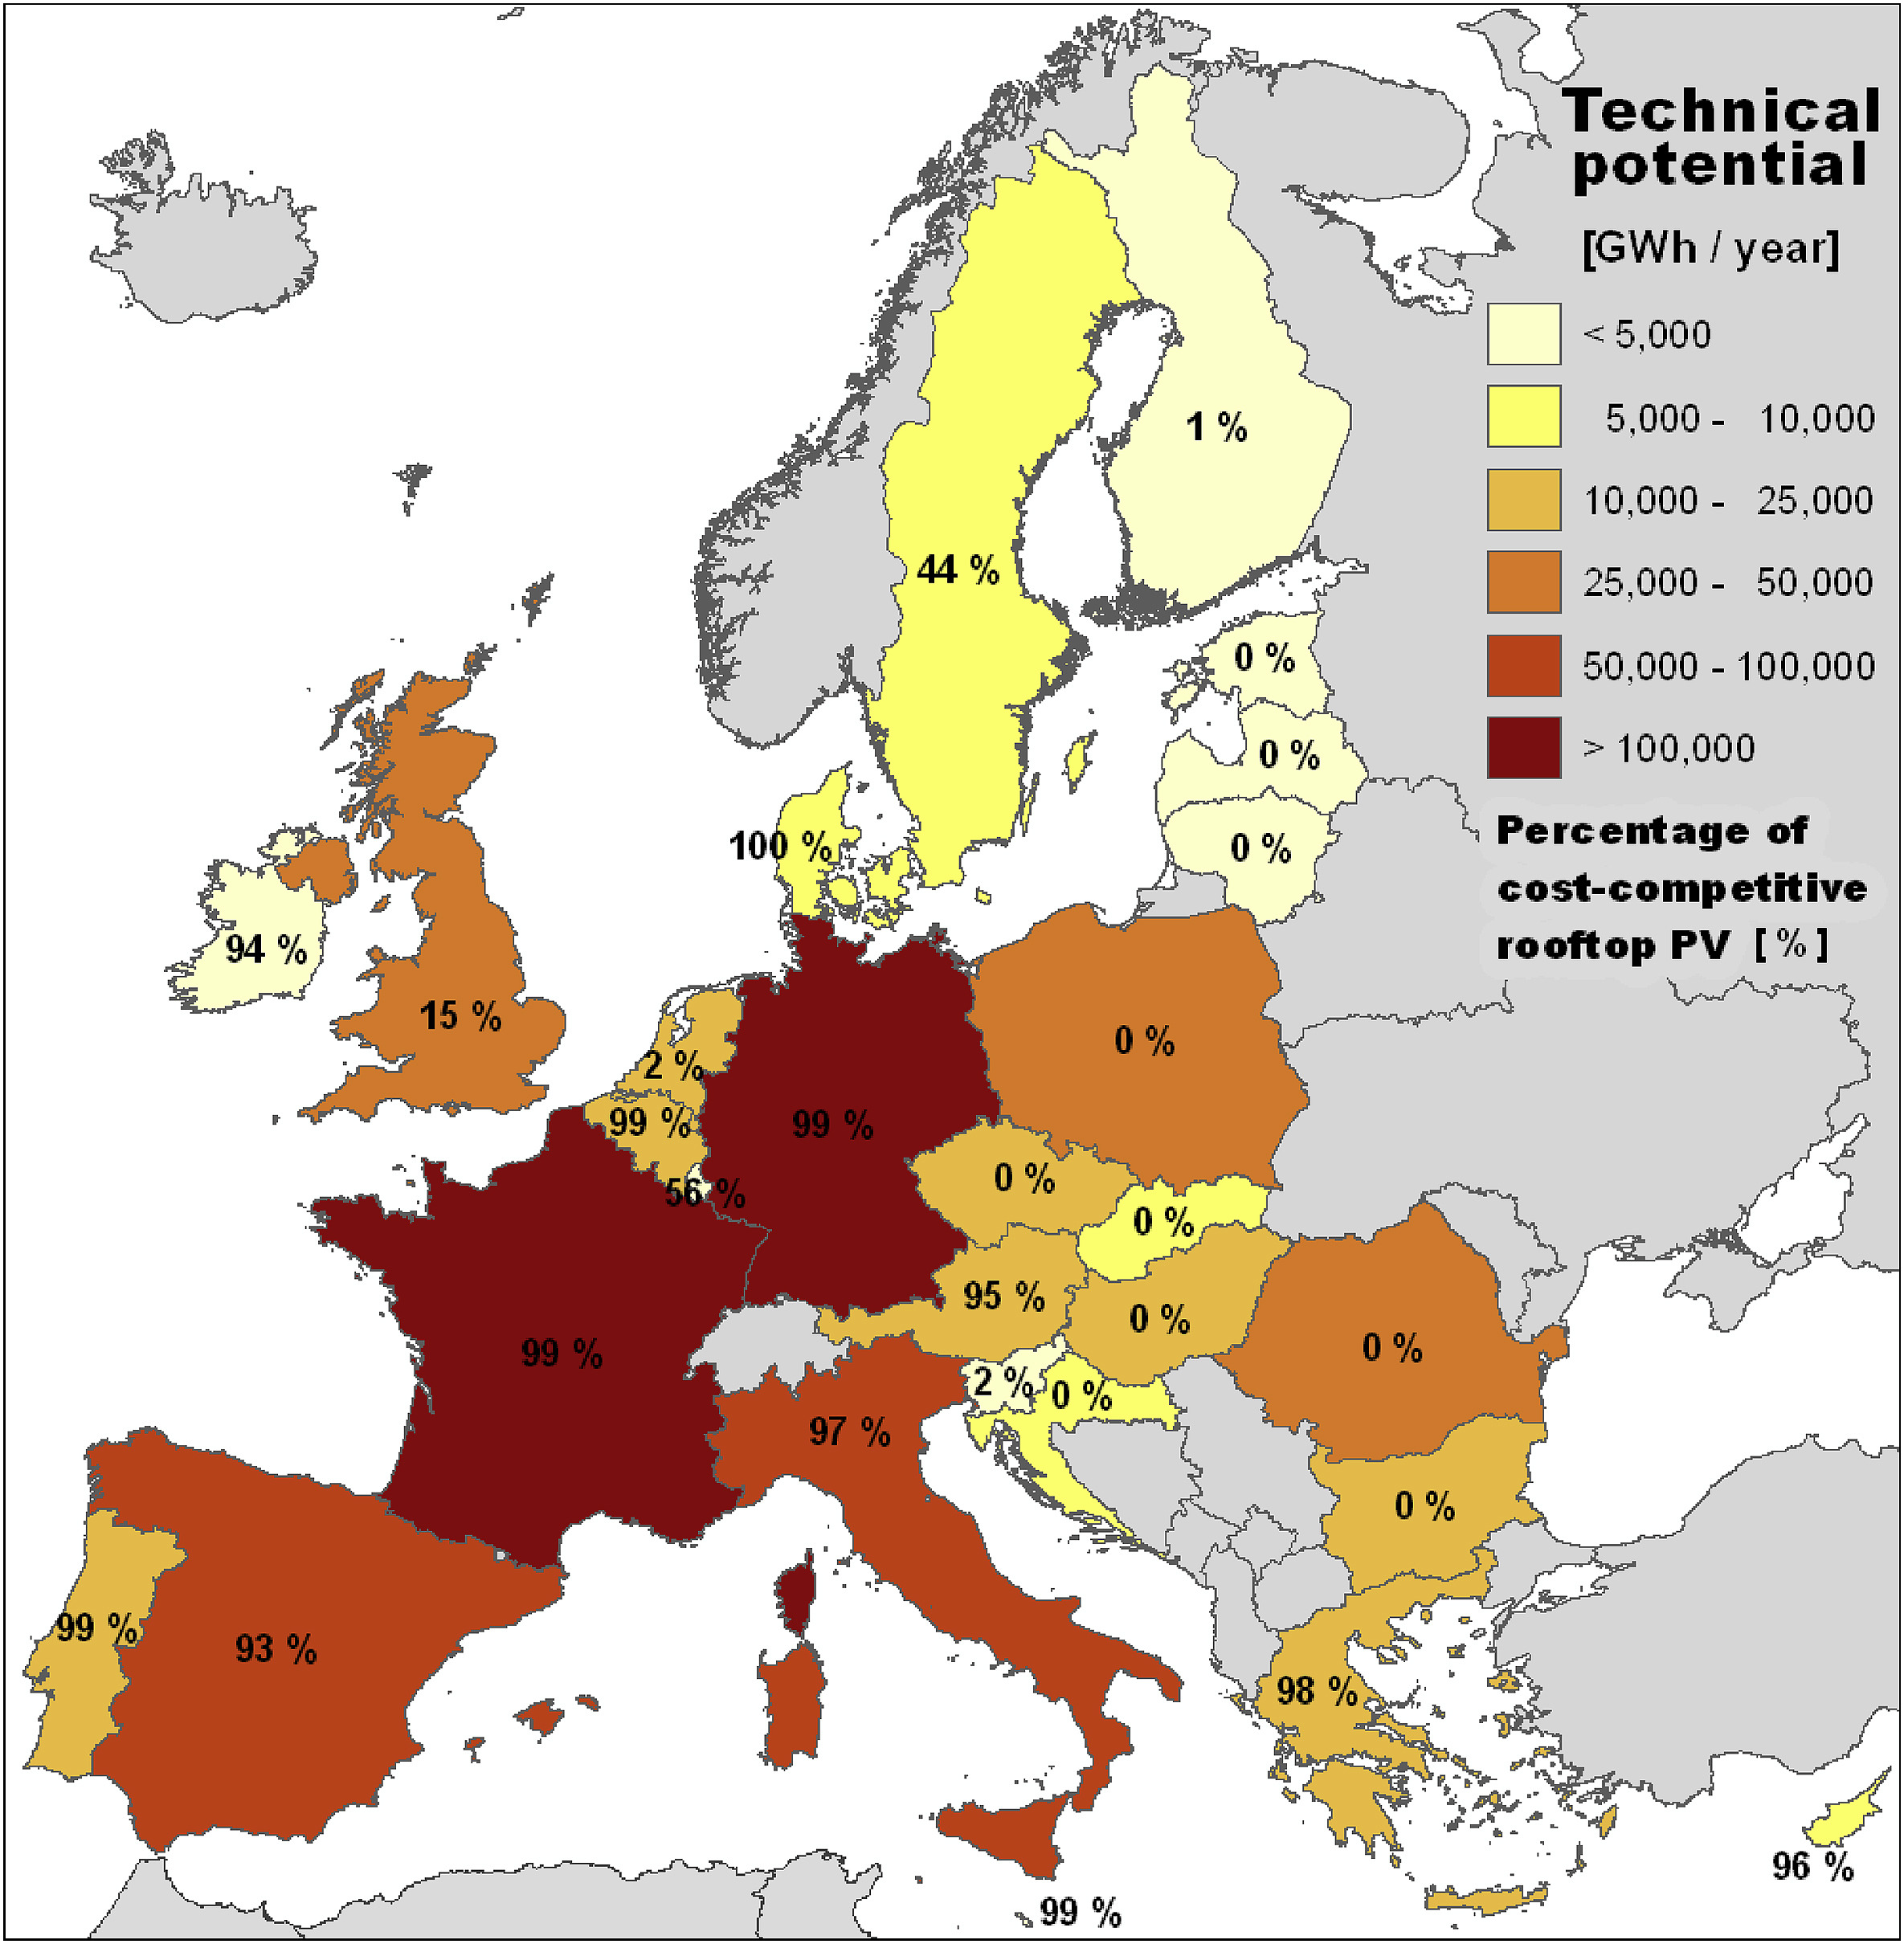
\includegraphics[width=0.7\linewidth]{../figures/technical_potential_eu.jpg}
\end{SCfigure}

\section*{Related work}
\citet{freitas2015modelling} present an overview of approaches combining algorithms and GIS modeling to estimate solar potential in dense urban environments. They compare different numeric solar radiation algorithms and data sources ranging from 2d maps to high resolution 3d models of urban scenes. In their survey, they find that major factors limiting these approaches include poor data quality and the difficulty of validating models.\\
\cite{bodis2019high} use high-resolution satellite data and statistical information to produce an estimate of solar potential across the whole EU. They also include economical calculations in their method to estimate viability of installing solar. However, their method only yields estimates for areas and not for specific rooftops.\\
Similar and very early approaches are proposed by \citet{ouammi2012artificial} and \citet{sozen2004use} who use rudimentary neural network architectures and focus on Moroccan and Turkish territory respectively. \citet{assouline2018large} focus on Switzerland and use random forests for their predictions.\\
With project sunroof, the technology company Google has proposed an approach that offers fine-grained solar potential estimation for individual rooftops within the United States and Puerto Rico. From Google Maps data, they find rooftop outlines using a (not further specified) deep learning method. They then estimate rooftop geometry and use historical weather data to predict the solar potential \cite{sunroof}.\\
Further private sector endeavors include a cooperation between the companies Otovo and In Sun We Trust that offer a product similar to Project Sunroof but only serve France \cite{insun}. Other existing products focus on small areas or only offer solar potential estimates on-demand \cite{insun, rhino}.\\
\citet{lee2019deeproof} propose a data-driven method that mostly relies on widely available satellite data. They estimate roof topology directly from this imagery using image segmentation architectures. They then use further public data of solar radiance to estimate solar potential. They validate their method by comparing it to a precise but expensive LIDAR-based approach. Their method can be applied in a wide variety of settings.\\
Several other approaches leveraging sophisticated deep learning methods are proposed for solar potential estimation \cite{huang2019urban, zhong2021city} or solar irradiance mapping \cite{kumari2021deep, chandola2020multi, bamisile2020application}.


\section*{Method}
\begin{figure}
	\centering
	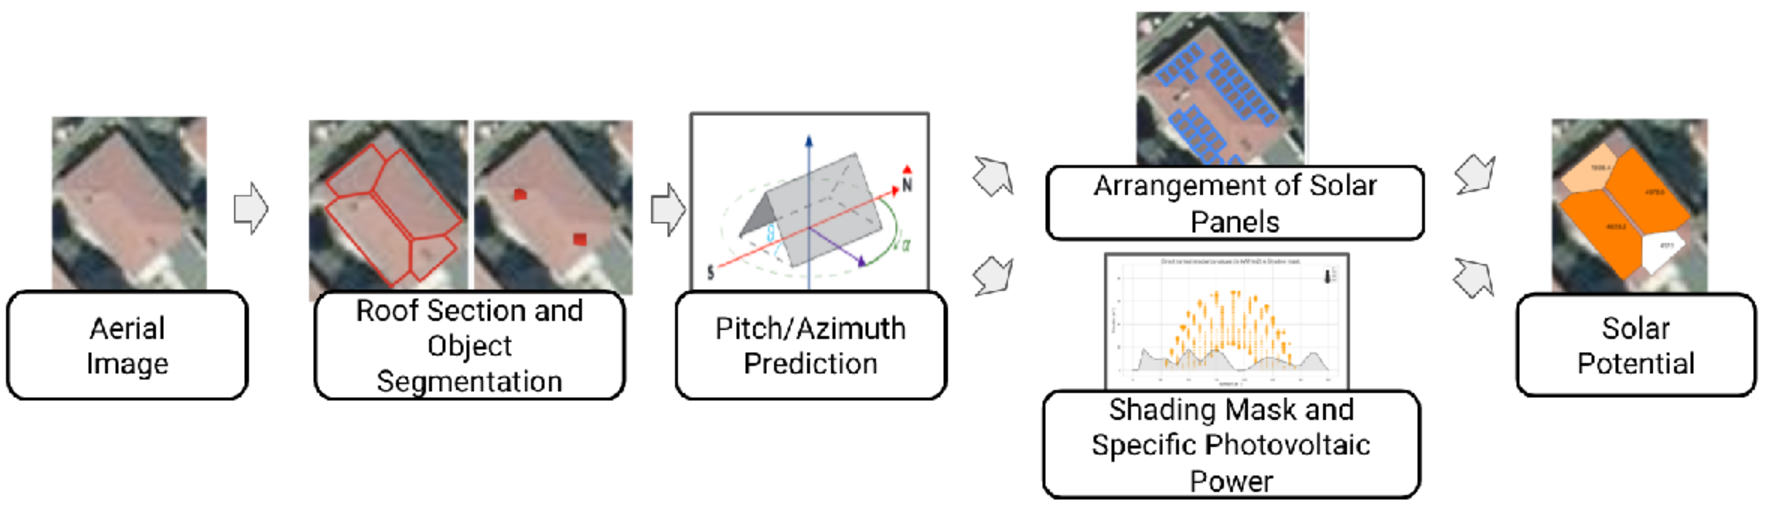
\includegraphics[width=\linewidth]{../figures/fig_1.pdf}
	\caption{The figure is taken from \citet{de2021predicting}}
	\label{fig:arch}
\end{figure}
With the challenges of large-scale solar potential for individual rooftops established and several related proposed methods established, we will use this section to explain the method proposed by \citet*{de2021predicting} in detail. The major steps are illustrated in \figref{fig:arch}.\\
\subsection*{Segmentation}
Given satellite imagery, \citet{de2021predicting} first identify suitable roof spaces. This includes finding roof and more precisely, sections of roofs where solar panels can be installed. This means omitting ridges or occupied roof spaces. Therefore, they segment into the categories background, sections, ridges, and roof objects. They use two different models to achieve this. \cite{de2021predicting}\\
To extract features from raw images, they use a ResNet backbone \cite{he2016deep} with 34 residual blocks.\\
Inspired by U-Net \cite{ronneberger2015u} they store features along the layers during encoding the input. When decoding the features they progressively concatenate these kept features with upsampled ones that match in dimension. This ensures that information from input images is not lost and the model rather has to learn a difference to the input image as opposed to a whole new image. Satellite imagery is particularly rich in structural information, such as sharp and straight outlines of roofs or roads.\\
To train the model, \citet{de2021predicting} use labels obtained from GIS data and manually annotated images from the French cities of Bordeaux, Brest, Montpellier, and Strasbourg.
%\citet{de2021predicting} obtain labels from 3d models


\subsection*{Geometry}
Once they obtain the segmentation maps where roof space suitable for solar panel installation is denoted as specific class, \citet{de2021predicting} regress on pitch and azimuth of such areas. This gives 3d information about the roofs geometry.\\
They pitch of a roof segment refers to its slope. This plays a crucial role for solar potential since roofs that are either completely flat or vertical might be less beneficial than a moderately sloped one. \citet{de2021predicting} regress on the normalized pitch. For this they use a simple linear regression algorithm \cite{gross2003linear}. The training data is obtained again from 3d models of the five French cities. Additionally,\citet{de2021predicting} use a random forest algorithm \cite{belgiu2016random} to predict roof inclination where features, such as roof type, material, and shape or the height of the building are known.\\
The azimuth refers to the orientation of the roof from a bird's view perspective. This is obviously important as i.e. on the northern hemisphere south facing segments might receive more solar radiation than otherwise oriented ones.\\ \citet{de2021predicting} compute it analytically. For this, they make the simplifying assumption that roof segment orientations can be assigned on of four classes which are the elements of a cyclic \SI{90}{\degree} rotation group. This allows them to treat it as a classification problem to which the solution can be obtained in closed form.

\subsection*{Panel Arrangement}
Based on the predicted roof section that is suitable for solar panel installation and its predicted geometry, \citet{de2021predicting} compute the maximum number of pannels that can be installed. Given the simple rectangular shape of solar panels, they are able apply a greedy algorithm to the problem. The algorithm's primary aim is to fit as many panels of a fixed size to a roof segment. It accounts for objects occupying rooftop space, mandatory distances between panels and to roof edges, and overlapping.



\subsection*{Shading}
A roofs shading depends on factors such as surrounding vegetation and buildings, its location and geometry, and meteorological factors. To compute the shading, a roof segment is objected to, \citet{de2021predicting} use the SkyViewFactor software \cite{zakvsek2011sky} to obtain data on how much light could reach the panels theoretically. This information is refined further using the R-package shadow \cite{dorman2019shadow}.\\
Additionally, \citet{de2021predicting} use digital elevation models and projected shadow computations using a QGIS extension \cite{qgis,qgisshadows} to produce a second shading mask per panel. \citet{de2021predicting} then combine the two shading masks for a final shading prediction.



\subsection*{Solar potential prediction}




\section*{Discussion}
- no real evaluation possible
- not end2end trainable
- not very scalable


\section*{Conclusion}


\newpage

\bibliographystyle{unsrtnat}
\bibliography{refs}

\end{document}
